\documentclass[main.tex]{subfiles}
\setdoublesep{0.35700 em}  % 'Bond Spacing'
\setatomsep{1.78500 em}    % 'Fixed Length'
\setbondoffset{0.18265 em} % 'Margin Width'
\newcommand{\bondwidth}{0.06642 em} % 'Line Width'
\setbondstyle{line width = \bondwidth}
\newcommand\chapterlabel{geometry}
\setcounter{figurenewcounter}{0}

\begin{document}

\linenumbers


\chapter[Electronic structure of molecules ]{Electronic structure of molecules}
\label{ch:bond}


   
    \begin{marginfigure}
\begin{tikzpicture} \node (a) at (0,0) {\includegraphics[width=4cm]{chapter6/figure1}} node[rotate=90, font=\tiny] at ([yshift=.5cm,xshift=.1cm]a.south east) {\textsuperscript{\textcopyright} PngImg} ;
\end{tikzpicture}
\label{fig:marginfig}
\end{marginfigure}
   
   
\lettrine[lines=4]{\color{black!45}M}{olecules} can found in a myriad of different shapes in nature. Some like carbon dioxide are one-dimensional or linear, other like methane have a three-dimensional shape. This chapter is devoted to the analysis of the molecular shape and to study more advanced models of the chemical bond. More importantly, this chapter is devoted to the reason why different molecules have different shapes: the molecular bond and the existence of lone pairs of electrons. You will be able to draw the connections between the atoms of a molecule.  The chemical bonds and the molecular geometry affect the properties of a molecule. At the end of the chapter we will address the polarity of molecules and you will understand the reasons why you use soap to get rid of oil while doing dished.

\begin{marginfigure}%LEARNING GOALS BOX
\begin{mytcbox}{GOALS}
\begin{enumerate}[label=\protect\circled{\color{white}\arabic*}]
\item Construct electron-dot structures
\item Identify the geometry of a molecule
\item Identify the polar character of a molecule
\item Calculate the bond hybridization 
 \item Interpret molecular orbital diagrams
\end{enumerate}
\end{mytcbox}
\vspace{1cm}

\begin{tcolorbox}[enhanced,colback=red!5!white,colframe=black!50!red,boxrule=1pt,
  arc=0pt,outer arc=0pt,drop heavy lifted shadow]
\faGears\ 
\docenvdef{Discussion:} oil spills on your shirt during a dinner. List three chemicals than can remove the stain  \end{tcolorbox}


\end{marginfigure}%LEARNING GOALS BOX

\section{Electron-dot structures of atoms}
Atoms are made of protons, neutrons and electrons. Electrons--in particular valence electrons--are responsible for the main chemical properties of an atom. These electrons are weakly tied to the nucleus in comparison with the core electrons and hence they can be exchanged. Atoms in a molecule, with a few exception, tend to be surrounded by eight electrons so that its electron configuration resembles a noble gas. This is known as the octet rule, and this is the reason why atomic F ($[He]2s^22p^5$) can easily receive an extra electron producing ionic \ce{F^-} ($[He]2s^22p^6$=[Ne]) or atomic Na ($[Ne]3s^1$) prefers to loose an electrons producing ionic \ce{Na^+} ($[He]2s^22p^6=[Ne]$). The electron-dot structure of an atom or a molecule is a visual representation of the electronic arrangement around an atom or in a molecule. 
\sloppy 
%\begin{marginfigure}%%%%%%%MARGIN FIGURE
%      \includegraphics{chapter6/figure2}
%      \label{fig:marginfig}
%      \caption{Valence electrons in a Ne atom}
%	\end{marginfigure}%%%%%%%MARGIN FIGURE
	
	

	
	
\begin{description}
\item[\docfilehook{Valence electrons}{Valence electrons}] The electrons of an atom can be divided in core electrons and valence electrons. The valence electrons of an atom are involved in chemical bonds as they are less bonded to the nucleus. The number of valence electrons in an atoms is the same as the group number. As an example, hydrogen \ce{H} belong to the group IA and hence has one valence electrons. Similarly, oxygen \ce{O} belongs to the group VIA and therefore it has six valence electrons.

\begin{example} %%%%%%%%%%%%%%%%%%%%%%%% EXAMPLE BOX
Indicate the number of valence electrons for the following atoms: N, O, C and S.\\
\textlcsc{ \textcolor{dgreen}{\Large \textbf{Solution}} }\\
Nitrogen is in group VA and hence it has five valence electrons (5\ce{e^-}). Oxygen belongs to the group VIA and C belong to IVA, hence they have 
\\
\faDiamond\ \textlcsc{ \textcolor{dgreen}{\Large \textbf{Study Check}} }\\
Indicate the number of valence electrons for the following atoms: Cl and B.\\
\flushright Answer: Cl (7\ce{e^-}), B (3\ce{e^-}).
\end{example}%%%%%%%%%%%%%%%%%%%%%%%% EXAMPLE BOX


\item[\docfilehook{The octet rule}{The octet rule}] Atoms gain or loose electrons when they combine to form molecules. The octet rule says that each atom in a molecule is surrounded by eight electrons. There are two important exceptions to this rule as \ce{H} is only surrounded by two electrons, and \ce{B} by six.
\item[\docfilehook{Electron-dot structure of an atom}{Electron-dot structure of an atom}] In order to write the electron-dot structure of an atom, you just need to write down the symbol of the atom surrounded by the number of valence electrons one by one four directions, and if you have more than four electrons then add remaining electrons as pairs. For example, oxygen has six valence electrons and hence, the electron-dot structure would be \hspace{.05in}\lewis{0:2:4.6.,O}\hspace{.05in} Similarly, for the case of fluorine the  the electron-dot structure would be  \hspace{.05in}\lewis{0:2:4:6.,F} \hspace{.05in} In the case of an ion, you need to add (if its an anion) or substract (if its a cation) electrons, and for example the electron-dot structure of \ce{O^{2-}} is \hspace{.05in}\lewis{0:2:4:6:,O}\hspace{.05in}\ce{^{2-}}
%\begin{marginfigure}%%%%%%%MARGIN FIGURE
%      \includegraphics{chapter6/figure3}
%      \label{fig:marginfig}
%      \caption{Lewis structure of C}
%	\end{marginfigure}%%%%%%%MARGIN FIGURE
\begin{example} %%%%%%%%%%%%%%%%%%%%%%%% EXAMPLE BOX
Write down the electron-dot structure for the following atoms: \ce{N}, \ce{C} and \ce{Cl^-}.\\
\textlcsc{ \textcolor{dgreen}{\Large \textbf{Solution}} }\\
N has five valence electrons, whereas C has four. Hence the electron-dot for both will be: \hspace{.05in}\lewis{0.2:4.6.,N}\hspace{.05in} and  \hspace{.05in}\lewis{0.2.4.6.,C}\hspace{.05in}. \ce{Cl^-} has eight valence electrons, that is seven plus one, and hence its electron-dot structure will be \hspace{.05in}\lewis{0:2:4:6:,Cl}\hspace{.05in}\ce{^{-}}. \\
\faDiamond\ \textlcsc{ \textcolor{dgreen}{\Large \textbf{Study Check}} }\\
Write down the electron-dot structure for \ce{N^{3-}}\\
\flushright Answer: \hspace{.05in}\lewis{0:2:4:6:,N}\hspace{.05in}\ce{^{3-}}.
\end{example}%%%%%%%%%%%%%%%%%%%%%%%% EXAMPLE BOX


\item[\docfilehook{Electron-dot structure of diatomic molecules}{Electron-dot structure of diatomic molecules}] Now we will address how to build up electron-dot structures of molecules. The first step is (a) to set up the atoms in the molecule in the form of a line. After that, (b) you need to count the total number of valence electrons in the molecule, by adding the valence electrons of each atoms. Then you (c) calculate the pairs of electrons--the total number of valence electrons divided by two; pairs of electrons are represented by lines. In the following (d) you need to start distributing the pairs in the molecule in a very specific way: first connecting the surrounding atoms to the central atom, after placing pairs on top of the surrounding atoms and finally by placing the remaining pairs in the central atom. Each atom should be surrounded by four pairs with the exception of \ce{H} and \ce{B}.


\begin{example} %%%%%%%%%%%%%%%%%%%%%%%% EXAMPLE BOX
Construct the electron-dot structure of \ce{HCl}.\\
\textlcsc{ \textcolor{dgreen}{\Large \textbf{Solution}} }\\
\begin{enumerate}[label=\protect\circled{\color{white}\arabic*}]
\item \begin{bf}Step one:\end{bf} we first arrange the atoms in the molecule as \ce{H}\hspace{.05in}\ce{Cl}. 
\item \begin{bf}Step two:\end{bf} now we count the number of valence electrons: H(1) and Cl(7) that gives a total of eight electrons.
 \item \begin{bf}Step three:\end{bf} let us count the pairs of electrons; we have eight electrons and that is four pairs.
\item \begin{bf}Step four:\end{bf} now we distribute the pair on each atoms knowing that each atom has to have four pairs with the exception of hydrogen that can only be surrounded by one pair.
\lewis{0:,H}\hspace{.05in}\lewis{0:2:6:,Cl}\hspace{.05in}, using lines instead of pairs (this is not necessary but makes the electron-dot structure look better) we obtain\\
 \chemfig{ H-[:0]\lewis{026,Cl}}\hspace{.05in}.
\end{enumerate}
\faDiamond\ \textlcsc{ \textcolor{dgreen}{\Large \textbf{Study Check}} }\\
Construct the electron-dot structure of \ce{HF}.\\
\flushright Answer: \chemfig{ H-[:0]\lewis{026,F}}\hspace{.05in}.
\end{example}%%%%%%%%%%%%%%%%%%%%%%%% EXAMPLE BOX

\item[\docfilehook{Electron-dot structure of general molecules}{Electron-dot structure of general molecules}] Now we will address how to build up electron-dot structures of more complex molecules. The first step is (a) to arrange the atoms in the molecule, in the form of a central atom and the remaining atoms around it; the central atom is the one with a lower index in the molecule (e.g. in \ce{H2O} is \ce{O} or in \ce{NH3} is \ce{N}). After that, (b) you need to count the total number of valence electrons in the molecule, by adding the valence electrons of each atoms. Then you (c) calculate the pairs of electrons--the total number of valence electrons divided by two; pairs of electrons are represented by lines. In the following (d) you need to start distributing the pairs in the molecule in a very specific way (this is the key to building good electron-dot structures): first connecting the surrounding atoms to the central atom, after placing pairs on top of the surrounding atoms and finally by placing the remaining pairs in the central atom. Each atom should be surrounded by four pairs (this is the octet rule) with the exception of \ce{H} and \ce{B} as they do not follow the octet rule. When you have the final electron-dot structure, the pairs of electrons (or lines) that connect two atoms are called \begin{it}bonds\end{it}, whereas the pairs not involved in an connection are called \begin{it}lone pairs\end{it}. A very important note is that, at this point, is not that important the atom arrangement (if the molecule looks like a line, a triangle or so) as long as the connectivity (which atom goes in the center and in the surroundings) is correct. 

\begin{example} %%%%%%%%%%%%%%%%%%%%%%%% EXAMPLE BOX
Construct the electron-dot structure of \ce{H2O} indicating the number of bonds and lone pairs.\\
\textlcsc{ \textcolor{dgreen}{\Large \textbf{Solution}} }\\
\begin{enumerate}[label=\protect\circled{\color{white}\arabic*}]
\item \begin{bf}Step one:\end{bf} we first arrange the atoms in the molecule as \ce{H}\hspace{.05in}\ce{O}\hspace{.05in}\ce{H}. The central atom is \ce{O} as oxygen has the lower index in the \ce{H2O} molecule--the index for O is one and the index for H is two.
\item \begin{bf}Step two:\end{bf} now we count the total number of valence electrons, including all atoms: 2xH(1) and O(6) that gives a total of eight electrons.
 \item \begin{bf}Step three:\end{bf} let us count the pairs of electrons; we have eight electrons and that is four pairs.
\item \begin{bf}Step four:\end{bf} now we distribute the pair on each atoms knowing that each atom has to have four pairs with the exception of hydrogen that can only be surrounded by one pair.
\lewis{0:,H}\hspace{.05in}\lewis{0:2:6:,O}\hspace{.05in}\lewis{0:,H}\hspace{.05in} and using lines instead of pairs (this is not necessary but makes the electron-dot structure look better) we obtain \chemfig{ H-[:0]\lewis{26,O}-H}\hspace{.05in}. The molecule has two bonds, each one connecting and H to the oxygen atom and two lone pairs located on the oxygen atom.
\end{enumerate}
\faDiamond\ \textlcsc{ \textcolor{dgreen}{\Large \textbf{Study Check}} }\\
Construct the electron-dot structure of \ce{NH3} indicating the number of bonds and lone pairs..\\
\flushright Answer: \chemfig{\lewis{2,N}( (-[:0]H)(-[:180]H)(-[:270]H))}; three bonds and one lone pair.
\end{example}%%%%%%%%%%%%%%%%%%%%%%%% EXAMPLE BOX

\item[\docfilehook{Atomic charges in a molecule}{Atomic charges in a molecule}] In order to build up the electron-dot structures of a molecule you needs to count the number of valence electrons. Each atom bring a different number of valence electrons to a molecule. For example, H brings one whereas O brings two. When you arrange the electron pairs in the molecule, each atoms should have the number of electrons that they bring. For example in this electron-dot structure \lewis{0:,H}\hspace{.05in}\lewis{0:2:6:,Cl}\hspace{.05in} the hydrogen atom brings one electrons to the molecule, and in the molecule the atom owns one electrons, as in \lewis{0:,H}\hspace{.05in}  one of the dots belong to \ce{H} and the other belongs to the \ce{Cl}--the electrons are shared in a covalent bond. In the same way, the \ce{Cl} atom brings seven electrons and in the molecule it owns seven electrons, and has six electrons here \lewis{0:2:6:,Cl}\hspace{.05in} plus the one that shared with the hydrogen atom. In another words, the \lewis{0:,H}\hspace{.05in}\lewis{0:2:6:,Cl}\hspace{.05in} electron-dot structure is the combination of \lewis{0.,H}\hspace{.05in} and \hspace{.05in}\lewis{0:2:4.6:,Cl}\hspace{.05in}. We say that the charges on each atom are zero, as each atom in the molecule owns the same number of electrons that it originally brings.
\begin{example} %%%%%%%%%%%%%%%%%%%%%%%% EXAMPLE BOX
Indicate the atomic charges on each of the atoms of \chemfig{\lewis{2,C}( (-[:0]H)(-[:180]H)(-[:270]H))} \\
\textlcsc{ \textcolor{dgreen}{\Large \textbf{Solution}} }\\
The carbon atoms brings four electrons and in the molecule it is surrounded by eight electrons, five of which belongs to it. Hence the charge of C is $-1$; this means that carbon has one extra electron. Each hydrogen brings one electron and in the molecule each hydrogen has one electron (they share two electrons with C, one for C and one for H). \\
\faDiamond\ \textlcsc{ \textcolor{dgreen}{\Large \textbf{Study Check}} }\\
Indicate the atomic charges on each of the atoms of \chemfig{\lewis{26,N}( (-[:0]H)(-[:180]H))}\\
\flushright Answer: H(0) and N(-1). \chemfig{\lewis{26,N}\scriptstyle\ominus( (-[:0]H)(-[:180]H))}
\end{example}%%%%%%%%%%%%%%%%%%%%%%%% EXAMPLE BOX


\item[\docfilehook{Multiple bonds}{Multiple bonds}] Often times you are going to encounter electron-dot structures like\hspace{.05in} \chemfig{\lewis{4:,N}~\lewis{0:,N}}\hspace{.05in} in which the atoms are connected by means of a triple bond. You will also encounter double bonds \hspace{.05in} \chemfig{\lewis{3:5:,O}=\lewis{1:7:,O}}\hspace{.05in}  and single bonds. These are called multiple bonds and are formed while constructing electron-dot structures in order to avoid having atoms with atomic charges different than zero. Charged atoms in a molecule are in general not favorable. When you build electron-dot structures and you end up having large atomic charges, you can avoid that by moving electrons from the atom into the bond, hence creating multiple bonds.



\begin{example} %%%%%%%%%%%%%%%%%%%%%%%% EXAMPLE BOX
Construct the electron-dot structure of \ce{O2}.\\
\textlcsc{ \textcolor{dgreen}{\Large \textbf{Solution}} }\\
\begin{enumerate}[label=\protect\circled{\color{white}\arabic*}]
\item \begin{bf}Step one:\end{bf} we first arrange the atoms in the molecule as \ce{O}\hspace{.05in}\ce{O}\hspace{.05in}.
\item \begin{bf}Step two:\end{bf} now we count the total number of valence electrons, including all atoms: 2xO(6) that gives a total of twelve electrons.
 \item \begin{bf}Step three:\end{bf} let us count the pairs of electrons; we have twelve electrons and that is six pairs.
\item \begin{bf}Step four:\end{bf} now we distribute the pairs, fist connecting the atoms \chemfig{O-O} (we have five extra pairs to distribute at this point).
\item \begin{bf}Step five:\end{bf} we place the remaining pairs on top of the oxygen atoms \hspace{.05in}\chemfig{\lewis{246,O}-\lewis{17,O}}
\item \begin{bf}Step six:\end{bf} now we calculate the charge on each atom \hspace{.05in}\chemfig{\lewis{246,O}\scriptstyle\ominus - \scriptstyle\oplus\lewis{17,O}}
\item \begin{bf}Step seven:\end{bf} in order to eliminate the charges we move lone pairs into the bond \hspace{.05in}\chemfig{\lewis{35,O}=\lewis{17,O}}\hspace{.05in} Now the charges are zero and this is more important than imposing the octet rule.
\end{enumerate}
\faDiamond\ \textlcsc{ \textcolor{dgreen}{\Large \textbf{Study Check}} }\\
Construct the electron-dot structure of \ce{CO2}.\\
\flushright Answer: \hspace{.05in}\chemfig{\lewis{35,O}=\lewis{,C}=\lewis{17,O}}
\end{example}%%%%%%%%%%%%%%%%%%%%%%%% EXAMPLE BOX



\end{description}





\section{Molecular shape}
Molecules are arrangements of atoms, and these arrangements can be presented in different form. Let us use as an example the \ce{H2O} molecule, which contains two hydrogen atoms and one oxygen. Knowing that both hydrogens are connected to oxygen by means of a covalent bond, one can envision several molecular geometries such as \hspace{.05in} \chemfig{ H-[:0]\lewis{26,O}-H}\hspace{.05in} or maybe \hspace{.05in}\chemfig{ H-[:45]\lewis{26,O}-[:315]H}\hspace{.05in}. The goal of this section is to identify the geometry of a given molecule. In order to do this, the electron-dot structure of the molecule are the key.
%\begin{marginfigure}%%%%%%%MARGIN FIGURE
%      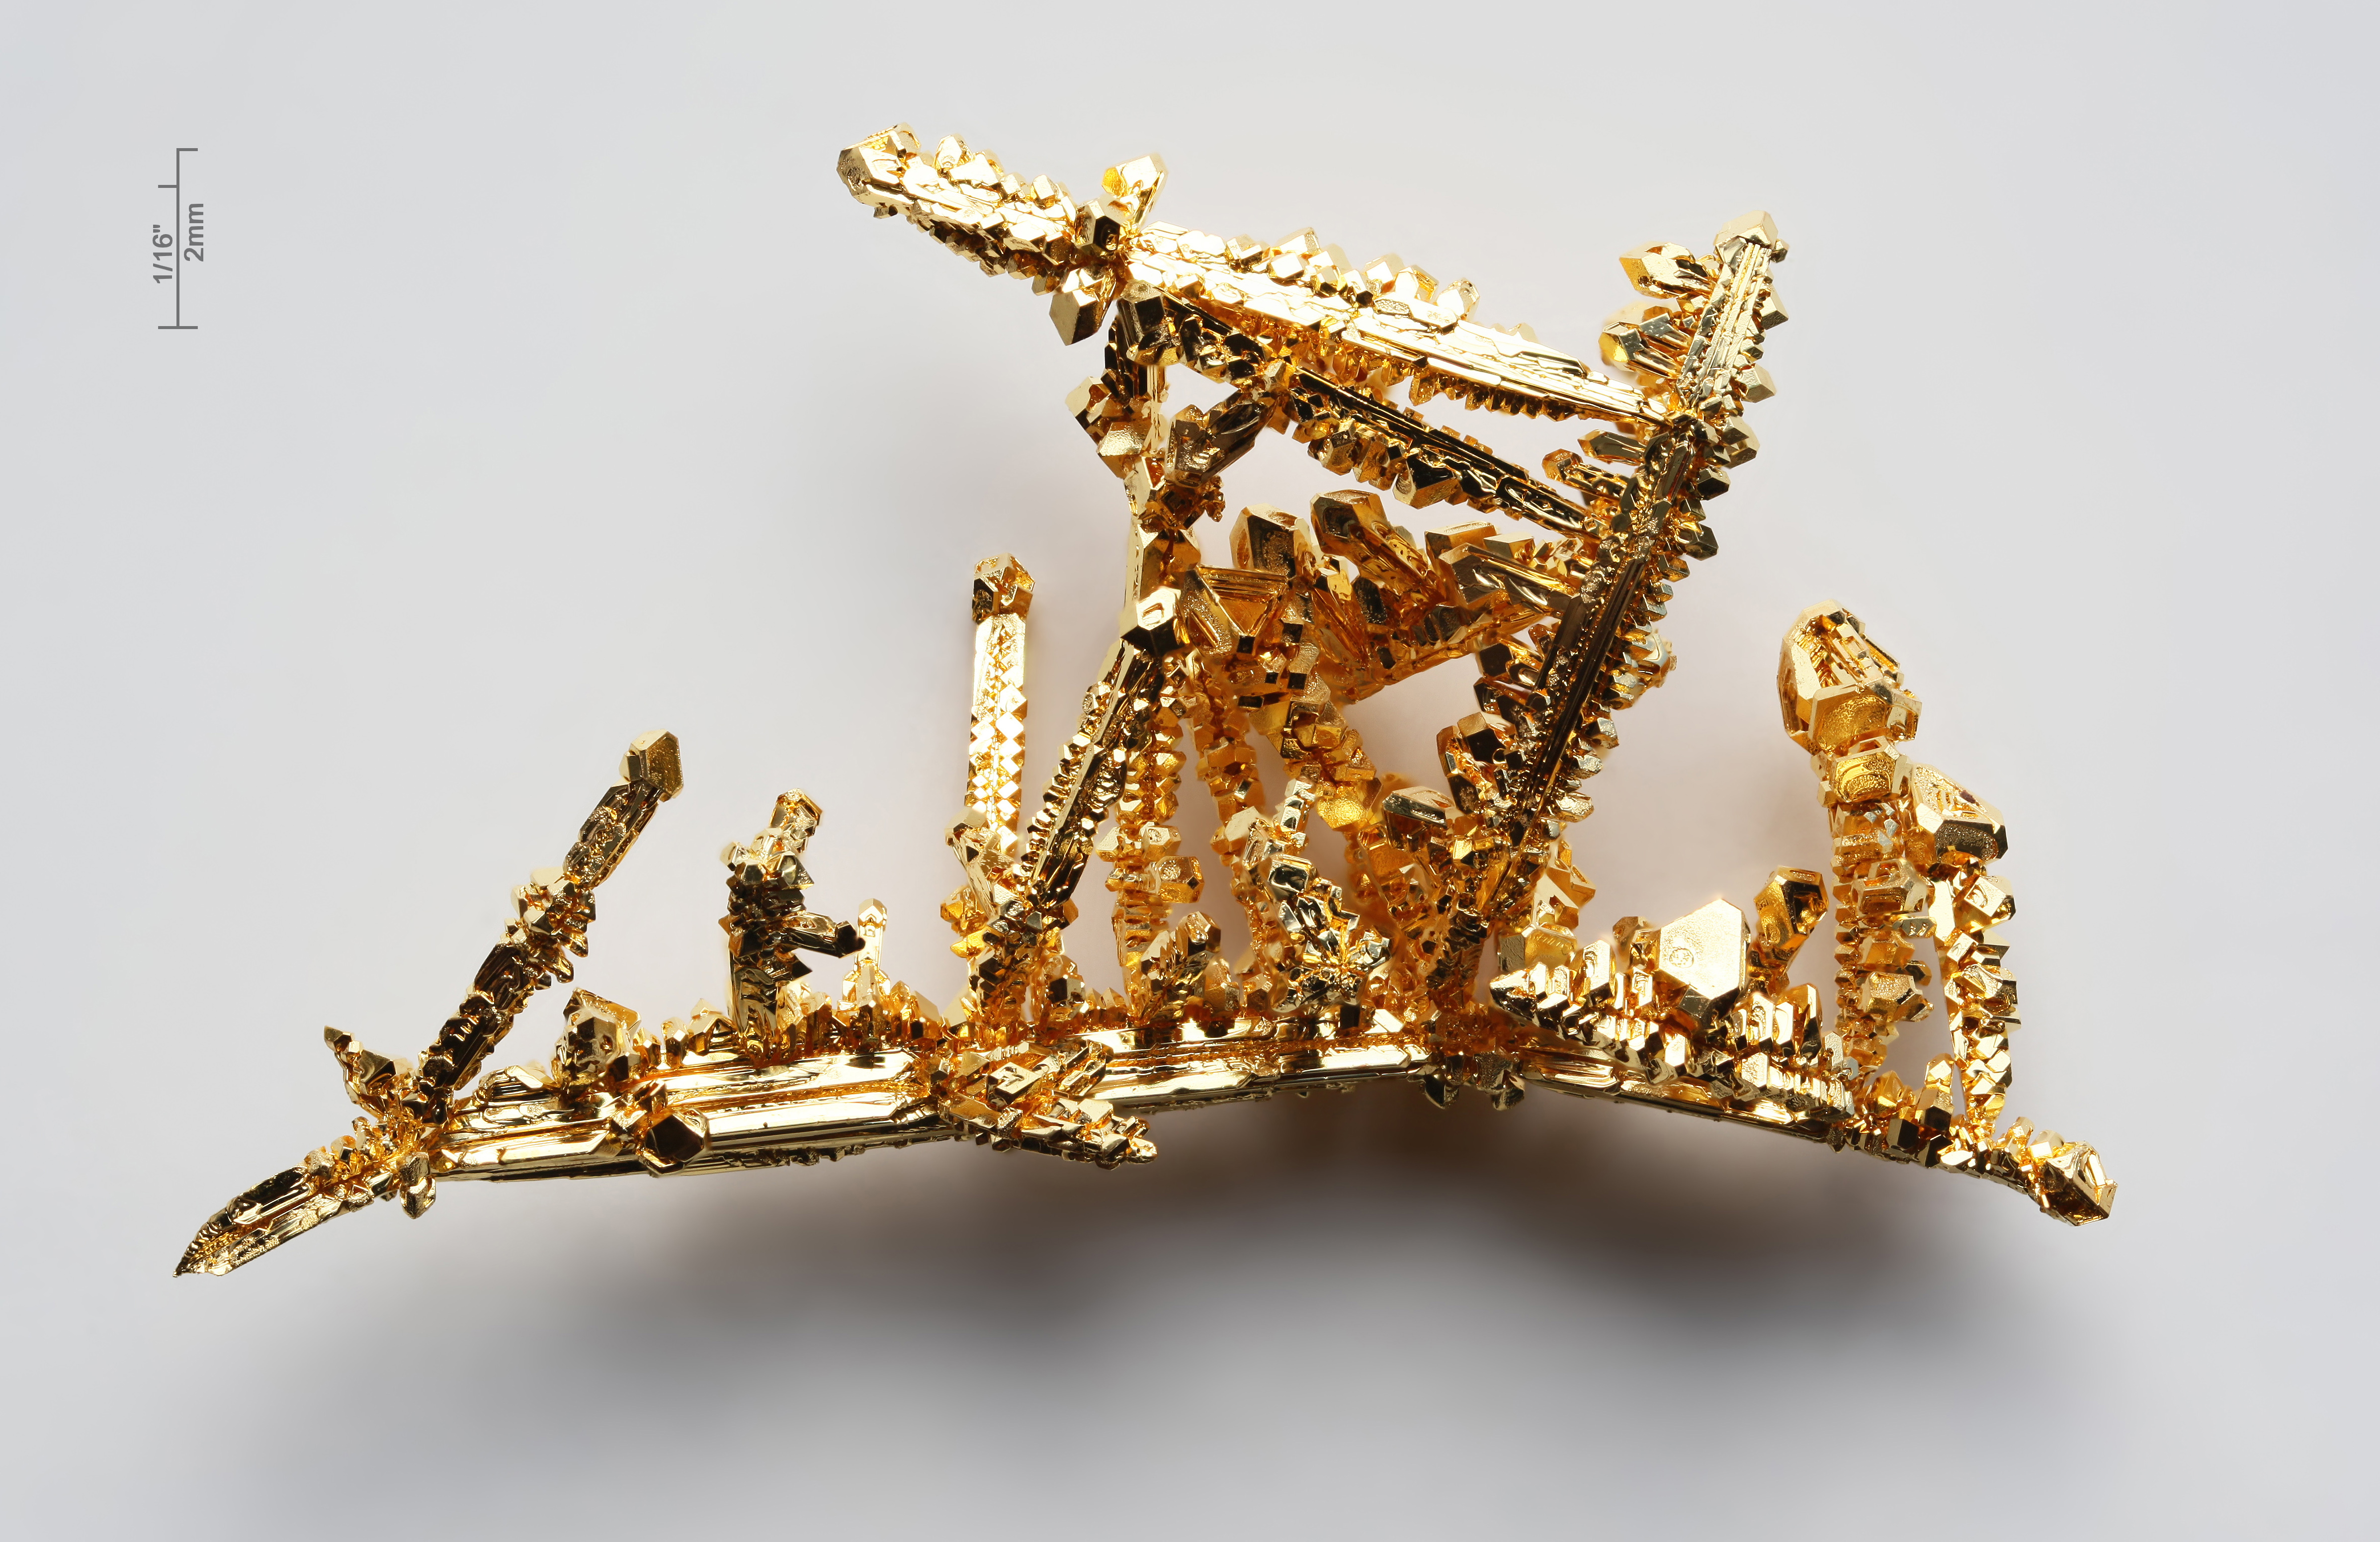
\includegraphics{chapter6/figure6}
%      \label{fig:marginfig}
%      \caption{tetrahedral molecule}
%	\end{marginfigure}%%%%%%%MARGIN FIGURE
\sloppy 
\begin{description}
\item[\docfilehook{ABE Molecular code}{ABE Molecular code}] If the molecule contains two atoms, there is only a possible geometry these two atoms can exhibit, and this is a linear arrangement. For the case of more complex molecules, in order to identify the geometry you need to figure out the ABE code of the molecule. In this code B refers to the number of atoms connected to the central atom in a molecule, and E is the number of lone pairs on the central atom. For example, the electron-dot \hspace{.05in}\chemfig{ H-[:0]\lewis{26,O}-H}\hspace{.05in} structure has two bonds with the central atom \ce{B2} and two lone pairs on top of the central atom \ce{E2} and hence the ABE code of the molecule would be \ce{AB2E2}. Another example the ABE code for  ammonia  \hspace{.05in} \chemfig{\lewis{2,N}( (-[:0]H)(-[:180]H)(-[:270]H))} \hspace{.05in}  would be \ce{AB3E}, as the molecule has three atoms connected to the central nitrogen and and \ce{N} has a single lone pair. You can find a list of the equivalence between ABE codes and the molecular geometry in Table \ref{tab:vsepr}. In order to predict the geometry of a molecule, once you have the ABE code, Table \ref{tab:vsepr} will give you the geometry. For example, an \ce{AB2} molecule will be linear, whereas an \ce{AB2E2} is bent. The bond angles are also indicated in the table, and for example a \ce{CO2} molecule, which will be linear will have a $180^{\circ}$ angle. This means both C-O bonds will form a line.



\hspace{-6cm}
\begin{minipage}[b]{1.\linewidth}
\begin{center}
\refstepcounter{table} \label{tab:{\chapterlabel}1}
\fontfamily{ppl}\selectfont
\begin{tabular}{llllllll}
\rowcolor{black!45}
\toprule
\multicolumn{8}{l}{\hypersetup{colorlinks,linkcolor={white}} \cellcolor{black}\color{white}\bfseries\small Table \ref{tab:{\chapterlabel}1} Molecular geometries } \\
\midrule
ABE Code & Molecular shape & Bond Angle & 3D model  & ABE Code & Molecular shape & Bond Angle & 3D model \\
\midrule
\ce{AB2} &  Linear      &  $180^{\circ}$    &   \begin{minipage}{.1\textwidth}\includegraphics[width=\linewidth, height=40mm]{./chapter6/geom1}\end{minipage}   & \ce{AB4E} &  see-saw      &   180$^{\circ}$,120$^{\circ}$, 90$^{\circ}$       &   \begin{minipage}{.1\textwidth}\includegraphics[width=\linewidth, height=40mm]{./chapter6/geom9}\end{minipage}\\\ce{AB3} &  Trigonal Planar      &  $120^{\circ}$    &   \begin{minipage}{.1\textwidth}\includegraphics[width=\linewidth, height=60mm]{./chapter6/geom2}\end{minipage}& \ce{AB3E2} &  T-shaped     &  90$^{\circ}$, 180$^{\circ}$       &   \begin{minipage}{.1\textwidth}\includegraphics[width=\linewidth, height=40mm]{./chapter6/geom10}\end{minipage}\\
\ce{AB2E} &  Bent      &  $120^{\circ}$    &   \begin{minipage}{.1\textwidth}\includegraphics[width=\linewidth, height=40mm]{./chapter6/geom3}\end{minipage}& \ce{AB2E3} &  Linear    & 180$^{\circ}$       &   \begin{minipage}{.1\textwidth}\includegraphics[width=\linewidth, height=40mm]{./chapter6/geom11}\end{minipage}\\

\ce{AB4} &  Tetrahedral      &  $109^{\circ}$    &   \begin{minipage}{.1\textwidth}\includegraphics[width=\linewidth, height=40mm]{./chapter6/geom4}\end{minipage} & \ce{AB5E} &  square pyramidal     &  90$^{\circ}$      &   \begin{minipage}{.1\textwidth}\includegraphics[width=\linewidth, height=40mm]{./chapter6/geom12}\end{minipage}\\

  \ce{AB3E} &  Trigonal pyramidal    &  $109^{\circ}$    &   \begin{minipage}{.1\textwidth}\includegraphics[width=\linewidth, height=40mm]{./chapter6/geom5}\end{minipage}   & \ce{AB4E2} &  square planar   & 90$^{\circ}$, 180$^{\circ}$       &   \begin{minipage}{.1\textwidth}\includegraphics[width=\linewidth, height=40mm]{./chapter6/geom13}\end{minipage}\\
\ce{AB2E2} &  Bent    &  $109^{\circ}$    &   \begin{minipage}{.1\textwidth}\includegraphics[width=\linewidth, height=40mm]{./chapter6/geom6}\end{minipage}   &        &       &       &       \\
\ce{AB5} &  trigonal bipyramidal    &  $90^{\circ}$, $120^{\circ}$,$180^{\circ}$    &   \begin{minipage}{.1\textwidth}\includegraphics[width=\linewidth, height=40mm]{./chapter6/geom7}\end{minipage}   &        &       &       &       \\

\ce{AB6} &  octahedral   &  $90^{\circ}$, $180^{\circ}$,$180^{\circ}$    &   \begin{minipage}{.1\textwidth}\includegraphics[width=\linewidth, height=40mm]{./chapter6/geom8}\end{minipage}   &        &       &       &       \\
\bottomrule
\end{tabular}\end{center}
\end{minipage}





%\resizeableyellownote{2.5}{1}{Add Table \ref{tab:vsepr} into your flashcard.}


\begin{example} %%%%%%%%%%%%%%%%%%%%%%%% EXAMPLE BOX
Identify the geometry of the following molecules: \ce{BF3} and \ce{SO2}.\\
\textlcsc{ \textcolor{dgreen}{\Large \textbf{Solution}} }\\
We need first the electron-dot structure of both molecules. For \ce{BF3} \hspace{.05in}\chemfig{B(-[:0]\lewis{026,F})(-[:90]\lewis{024,F})(-[:180]\lewis{246,F})}.\hspace{.05in} The code of this molecule is \ce{AB3} and hence its geometry would be trigonal planar. The correct way to draw the molecule respecting its geometry would be:\hspace{.05in}\chemfig{B(-[:0]\lewis{026,F})(-[:120]\lewis{024,F})(-[:240]\lewis{046,F})}\hspace{.05in}. The electron-dot structure for sulfur dioxide--remember this is covalent molecule--is \hspace{.05in}\chemfig{\lewis{2,S}(=[:0]\lewis{06,O})(=[:180]\lewis{246,O})}\hspace{.05in} and its class is \ce{AB2E}. Hence the molecular geometry is linear.\\
\faDiamond\ \textlcsc{ \textcolor{dgreen}{\Large \textbf{Study Check}} }\\
Identify and draw the geometry of methane (\ce{CH4}).\\
\flushright Answer: Tetrahedral \hspace{.05in}\chemfig{C(-[:90]H)(-[:341]H)(-[:225]H)(-[:200]H)}\hspace{.05in}
\end{example}%%%%%%%%%%%%%%%%%%%%%%%% EXAMPLE BOX
\end{description}


\section{Polarity of molecules}
This section deals with bond and molecule polarity. A chemical bond will be polar or nonpolar depending on the tendency of the atoms in a bond to attract the electrons the bond. Polar bonds results in the existence of a permanent dipole moment that makes a molecule polar. Polar molecules can interact with polar molecules and mix. 

%\begin{marginfigure}%%%%%%%MARGIN FIGURE
%      \includegraphics{chapter6/figure5}
%      \label{fig:marginfig}
%      \caption{Electrostatic potential for the \ce{H2O} molecule showing molecular regions of positive and negative charge}
%	\end{marginfigure}%%%%%%%MARGIN FIGURE
\sloppy 
\begin{description}
\item[\docfilehook{Bond polarity}{Bond polarity}] Let us compare two different molecules: \ce{H2} and \ce{HCl}. We say \ce{H2} is a non-polar molecule. The reason for this is that each atom in the covalent H-H bond equally share the electrons. Differently, \ce{HCl} is a polar molecule, as \ce{H} is an electropositive atom and \ce{Cl} is electronegative. That implies that in the H-Cl covalent bond each atoms shares the electrons in the bond differently. H will be less prone to attract the electrons and Cl would tend to attract the bond electrons more than H. The result would be that the electrons in the bond would belong more to Cl than to H. Another consequence is that the molecule would have a permanent dipole--a permanent charge distribution--result of a uneven charge distribution in the chemical bond. We represent excess of charge as on Cl as \chemfig{Cl\pol{-}}\hspace{.05in} and electron deficiency in H as  \chemfig{H\pol{+}}. 
The polarity of the bond is represented as:
\begin{center}
\chemfig{
        \chemabove[3pt]{H}{\scriptstyle +}(-[::270,0.5,,,draw=none]@{a})-
        \chemabove[3pt]{Cl}{\scriptstyle - }(-[::270,0.5,,,draw=none]@{b})
        }
\chemmove{
          \draw[|->, very thick] (a)--(b);
         }
\end{center}

\item[\docfilehook{Polarity of diatomic molecules}{Polarity of diatomic molecules}] Molecules can either be polar or non-polar. The polarity of diatomic molecules only depends on the nature of the atoms that forms the molecule. If the atoms in the molecule are the same (e.g. \ce{H2} or \ce{O2}), then the molecule would be non-polar. If the atoms are different then the molecule would be polar. Examples are \ce{H2} a nonpolar molecule and \ce{HCl} or \ce{HBr}, both polar molecules. You can apply the same concept to a bond inside a molecule. The C-O bond in a \ce{CO2} molecule is a polar covalent bond, as C and O have different electronegativities.
\item[\docfilehook{Polarity of larger molecules}{Polarity of larger molecules}] The polarity of larger molecules would depend on the molecular geometry. Let us analyze the case of \ce{CO2}. Each of the C-O bonds on the molecule are polar bonds. However, \ce{CO2} is a linear molecule  \hspace{.07in}\chemfig{\lewis{35,O}=\lewis{,C}=\lewis{17,O}}\hspace{.07in} and the polarity of each C-O bonds compensate so that at the end the molecule is polar. For the \ce{H2O} case, again, the H-O bond is polar. However, the molecule is bent and looks just like\hspace{.05in}\chemfig{ H-[:45]\lewis{26,O}-[:315]H}\hspace{.05in}. Both H-O bonds do not compensate as they point in different direction and the directions do not cancel out what makes the water molecule to be a polar molecule.




\begin{example} %%%%%%%%%%%%%%%%%%%%%%%% EXAMPLE BOX
Identify the polar character (polar/nonpolar) of the following molecules: \ce{BF3}, \ce{SO2} and \ce{CH4}.\\
\textlcsc{ \textcolor{dgreen}{\Large \textbf{Solution}} }\\
Let us analyze the geometries of the three molecules:\\
\hspace{.05in}\chemfig{B(-[:0]\lewis{026,F})(-[:120]\lewis{024,F})(-[:240]\lewis{046,F})}\hspace{.05in}\hspace{.05in}\chemfig{\lewis{2,S}(=[:330]\lewis{06,O})(-[:210]\lewis{246,O})}\hspace{.05in} and \hspace{.05in}\chemfig{C(-[:0]H)(-[:90]H)(-[:180]H)(-[:270]H)}\hspace{.05in}
\\
The bonds on \ce{BF3} and \ce{SO2} do not cancel out, as they do not point in opposite directions. Hence these two molecules are polar. On the other hand, the bonds on methane cancel each other out and hence even when the C-H bond is polar, the molecule would be non-polar.\\
\faDiamond\ \textlcsc{ \textcolor{dgreen}{\Large \textbf{Study Check}} }\\
Identify the polar character (polar/nonpolar) of the following molecules: \ce{O2} and \ce{NH3}.\\
\flushright Answer: \ce{O2} is non-polar and \ce{NH3} is polar.
\end{example}%%%%%%%%%%%%%%%%%%%%%%%% EXAMPLE BOX


\item[\docfilehook{Polarity and mixing}{Polarity and mixing}] 
When you mix two different liquids or even gases, polarity is the key for the mixing process. If the molecules have the same polar character they will be able to mix, whereas they will not mix when the polar character is different. This section will cover several examples of mixing an polarity.

\item[\docfilehook{Molecules with the same polarity}{Molecules with the same polarity}] Water (\ce{H2O}) is a polar molecule. The ABE type of water of \ce{AB2E2} and hence its geometry is bent. That means both H-O bonds, which are polar, do not compensate with each other. Hence, the molecule will have a dipole moment and hence will be polar. Methanol (\ce{CH3OH}) is a polar molecule as well. The central atom of the molecule (C) is connected to three hydrogens and a OH group. Hence this will be a polar molecule as one of the atoms attached to carbon is different. Both molecules, water and methanol, will mix as they have the same polarity. Methane (\ce{CH4}) is a nonpolar molecule, as the four polar C-H bonds compensate each other. Similarly, \ce{CCl4}, tetrachloro methene, is another nonpolar molecule, for the same reason. Both molecules, \ce{CH4} and \ce{CCl4} will mix together. As a general rule: molecules with the same polarity (polar-polar or nonpolar-nonpolar) will mix.

\item[\docfilehook{Molecules with the same polarity}{Molecules with the same polarity}] \ce{CCl4} is a nonpolar molecule, and \ce{H2O} is a polar molecule. As both have different polar character they will not mix together. If you mix water and \ce{CCl4}, tow phases will remain instead of a single mixed liquid phase.
As a general rule: molecules with different polarity (polar-nonpolar) will not mix. Another example will be water and oil. Water is polar, and oil is a nonpolar molecule. As a consequence these two molecules will not mix together. Soap has a polar and non-polar part. In order to remove oil from water, soap helps mixing both polar water and nonpolar oil.

\end{description}


\section{Hybrid orbitals}
Lewis structures are just representations of the bonds in a molecule. These representations are based on the localized electron bonding model, that assumes that molecules are made of atoms that share pairs of electrons. This section will addressed more advanced models. In particular hybrid orbitals are mixtures of atomic orbitals in a molecule. Atoms contains electrons and these electrons are located in atomic orbitals. We call these atomic orbitals as they belong to atoms. When a few atomic orbitals mix together, they hybridize, that is they mingle forming combinations of orbitals called hybrid. For example, when a $s$ orbital hybridizes with a a single $p$ orbitals, we obtain a hybrid $sp$ orbital. At the same time, the $s$ orbital can hybridize with two different $p$ orbitals forming a $sp^2$ hybrid orbital. Hybrid orbitals are just a continuation of lewis structures and one can only obtain the hybrid orbitals of an atom in a molecule by means of the lewis structure. Therefore, at this point is very important you master the construction of lewis structures. 
%\begin{marginfigure}[-6cm]%%%%%%%MARGIN FIGURE
%\begin{tikzpicture}
%\setOrbitalDrawing{{very thin,  shading=ball, draw=none}}
%\satom[name=C, color=white, opacity=0.5]{red/90/90/0/1,red/180/180/0/1 ,red/25/25/0/0.8,red/270/270/0/1 }
%\draw[thick, fill=gray, opacity=.2] (0,1.5) -- (1.2,0.4) -- (0,-1.3) -- (0,1.5) -- (-1.6,-0.1) -- (0,-1.3);
%\draw[ dashed, thin, opacity=.2] (1.1,0.4) -- (-1.7,-0.1) ;
%\fill (-1.8,-0.4) circle (0pt);  \orbital[pos = {(-1.6,-0.1)}, opacity=0.5]{s} \node [above,yshift=-2cm] {H};
%\fill (0,-1.7) circle (0pt) ; \orbital[pos = {(0,-1.7)}, opacity=0.5]{s} \node [above,yshift=-0.3cm, xshift=-1.6cm] {H};
%\fill (1.3,0.4) circle (0pt) ; \orbital[pos = {(1.3,0.4)}, opacity=0.5]{s} \node [above,yshift=0.1cm, xshift=1.3cm] {H};
%\fill (0,1.6) circle (0pt) ; \orbital[pos = {(0,1.6)}, opacity=0.5]{s} \node [above,yshift=1.4cm, xshift=0.1cm] {H};
%\end{tikzpicture}
%            \caption{The molecule \ce{CH4} with class \ce{AB4} has hybridization $sp^3$. Four atomic orbitals are combined.}
%	\end{marginfigure}%%%%%%%MARGIN FIGURE
\sloppy 
\begin{description}
\item[\docfilehook{From ABE  code to hybridization}{From ABE  code to hybridization}] In order to obtain the hybridization of an atomic center in a molecule we just need the \ce{ABE} code and Table \ref{tab:hybrid}. For example, if the code of a molecule is \ce{AB4}, the hybridization of the molecule will be $sp^3$. Similarly, if the class is \ce{AB3} the hybridization will be $sp^2$ and in this case an empty $p$ orbital will remain in the bond--mind there are three different $p$ orbitals: $p_x$, $p_y$ and $p_z$. Another example, would be a molecule with class \ce{AB}. In this case, the hybridization will be $sp$ and two empty $p$ orbital will remain in the bond. A final example would be a molecule with class   \ce{AB4E}. This time, the hybridization would be $sp^3d^2$. Mind that in general the number of hybrid orbitals correspond to adding the $E$ and $B$ from the class. For example,  \ce{AB4E2}, we have two $E$ and four $B$ with a total of six orbitals, hence we will need a $s$ , three $p$'s and two $d$'s.











%\resizeableyellownote{2.5}{1}{Add Table \ref{tab:hybrid} into your flashcard.}


\hspace{0cm}
\begin{minipage}[b]{1.\linewidth}
\begin{center}
\refstepcounter{table} \label{tab:{\chapterlabel}2}
\fontfamily{ppl}\selectfont
\begin{tabular}{lccp{3cm}lc}
\rowcolor{black!45}
\toprule
\multicolumn{5}{l}{\hypersetup{colorlinks,linkcolor={white}} \cellcolor{black}\color{white}\bfseries\small Table \ref{tab:{\chapterlabel}2} Equivalency between the ABE code and the orbital hybridization} \\
\midrule
ABE Code & Electron Regions & Hybrid & Shape&Bond Angle  \\
\midrule
\ce{AB2}, \ce{ABE} &  2     &  sp &\begin{minipage}{.1\textwidth}\begin{tikzpicture}
\satom[name=A, color=green!50!black]{red/180/180/0/1 ,red/0/0/0/1}
\end{tikzpicture}\end{minipage}   &   $180^{\circ}$  \\
\ce{AB3}, \ce{AB2E},\ce{ABE3} &  3    &  sp$^2$ &\begin{minipage}{.1\textwidth}  \begin{tikzpicture}
\satom[name=A, color=green!50!black]{red/180/180/0/1 ,red/25/25/0/0.8,red/-30/-30/0/0.9 }
\end{tikzpicture}
\end{minipage}   &   $120^{\circ}$  \\
\ce{AB4}, \ce{AB3E},\ce{AB2E2},\ce{ABE3}  &  4    &  sp$^3$ &\begin{minipage}{.1\textwidth}  
\begin{tikzpicture}
\satom[name=A, color=green!50!black]{red/90/90/0/1 ,red/-19/-19/0/.9, red/255/255/0/1, red/199/199/0/0.9}
\end{tikzpicture}
\end{minipage}   &   $109.5^{\circ}$  \\
\ce{AB5}, \ce{AB4E},\ce{AB3E2},\ce{AB2E3}  &  5    &  sp$^3d$ &\begin{minipage}{.1\textwidth}  
\begin{tikzpicture}
\satom[name=A, color=green!50!black]{red/90/90/0/1,red/180/180/0/1 ,red/25/25/0/0.8,red/-30/-30/0/0.9,red/270/270/0/1 }
\end{tikzpicture}
\end{minipage}   &   $90^{\circ}$ and $120^{\circ}$  \\
\bottomrule
\end{tabular}\end{center}
\end{minipage}

\begin{example} %%%%%%%%%%%%%%%%%%%%%%%% EXAMPLE BOX
Given the following Lewis structures, identify the hybridization of the central atom:
\begin{center}\hspace{.05in}\chemfig{B(-[:0]\lewis{026,F})(-[:120]\lewis{024,F})(-[:240]\lewis{046,F})}\hspace{.05in}\hspace{.15in}\chemfig{\lewis{2,S}(=[:330]\lewis{06,O})(-[:210]\lewis{246,O})}\hspace{.05in} and \hspace{.05in}\chemfig{C(-[:0]H)(-[:90]H)(-[:180]H)(-[:270]H)}\hspace{.05in}
\end{center}
\textlcsc{ \textcolor{dgreen}{\Large \textbf{Solution}} }\\
In order to identify the hybrid character of the central atom, we first need to obtain the \ce{ABE} code. For \ce{BF3} the class is \ce{AB3}, for \ce{SO2} is \ce{AB2E} and finally for \ce{CH4} is \ce{AB4}. The number of electron regions for \ce{BF3} is three. Therefore we would need three hybrid orbitals: $sp2$. An empty $p$ orbital will remain unused in the bond. For  \ce{SO2} we need three electron regions and hence the hybridization of the central atom will also be $sp2$. For the case of methane, the hybridization will be $sp3$, as the molecule has four electron regions.
\\
\faDiamond\ \textlcsc{ \textcolor{dgreen}{\Large \textbf{Study Check}} }\\
Identify the hybridization of the central atom for the following molecules: \ce{O2} and \ce{NH3}.\\
\flushright Answer: $sp$  and $sp3$.
\end{example}%%%%%%%%%%%%%%%%%%%%%%%% EXAMPLE BOX





\end{description}





\section{Molecular orbital theory}
The molecular orbital theory is the most advanced bonding theory able to describe bond energies and bond lengths. Atomic orbitals are waves. When combining two waves one can obtain two possible results: a constructive combination and destructive combination. The molecular orbital theory assumes that atomic orbitals combine to form molecular orbitals. For every two atomic orbitals you can obtain two possible molecular orbitals: one is called bonding orbital, result from the constructive combination, and an other one called antibonding orbital, resulting from the destructive combination. In this section we will learn how to interpret molecular orbital diagrams.
   
    
%\begin{marginfigure}%%%%%%%MARGIN FIGURE
%\pgfplotsset{
%  axis lines=middle,
%  axis line style={->},
%  xmin=0,
%  xmax=4.2*pi,
%  xticklabels=empty,
%  xtick=\empty,
%  ymin=-1,
%  ymax=1,
%  yticklabels=empty,
%  ytick=\empty,
%  samples=200,
%  domain=0:4*pi,
%  every axis plot post/.append style={very thick},
%  clip=false
%             }% end of common axis set
%    \begin{tikzpicture}[scale=0.5]
%\begin{axis}% 1. plot
%[yscale=0.5]
%\addplot[red] {(sin(deg(x)))};
%\node at (2*pi,-1.05) {\huge$+$};
%\end{axis}
%\begin{axis}% 2. plot
%[ yshift=-3cm, yscale=0.5]
%\addplot[blue] {(sin(deg(x)))};
%\node at (2*pi,-1.05) {\huge$=$};
%\end{axis}
%    \end{tikzpicture}
%   
%    \begin{tikzpicture}[scale=0.5]
%\begin{axis}% 3. plot
%\addplot[purple] {(sin(deg(x)))};
%\end{axis}
%    \end{tikzpicture}
%    \hfill %%%% %%%% %%%% second image
%   \caption{Constructive combination of two waves. The combination results in a higher intensity wave.}
%	\end{marginfigure}%%%%%%%MARGIN FIGURE
     
     
	
	
    \sloppy 
\begin{description}


\item[\docfilehook{Bonding and antibonding orbitals}{Bonding and antibonding orbitals}] Atomic orbitals (AOs) combine to produce molecular orbitals (MOs). The combination of two atomic orbitals results in two new molecular orbitals: a bonding orbital and a antibonding orbital. Bonding MOs are more stable than the corresponding atomic orbitals. Antibonding MOs are less stable--they have a higher more positive energy--than the corresponding AOs. Antibonding orbitals are normally labeled with a $^*$ sign. Let us analyze both combinations of a $1s$ orbital. We can add both $1s$ orbital and the result is a bonding orbital, or we can substract both $1s$ orbitals and the result is an antibonding orbital, as the electron density cancels.



\stepcounter{figurenewcounter}   \refstepcounter{figure}  \label{Fig:{\chapterlabel}\thefigurenewcounter}
     \begin{center}

\begin{tikzpicture} [transform canvas={rotate=-0, shift={(-5em,0em)}}]
\begin{scope}[->,xshift=-1.9cm]
      \draw(0,0,0)coordinate(O)--+(.5,0,0)node[above]{\tiny\(x\)};
      \draw(O)--+(0,.5,0)node[above]{\tiny\(y\)};
      \draw(O)--+(0,0,.5)node[left]{\tiny\(z\)};
    \end{scope}
\begin{scope}[xshift=0cm]
\node[scale=0.5] at (0.0,0.0) {\usebox\mononut} ;\node at (0,-1.0) {$1s$};\node at (1.0,0.0) {\huge$+$};
;\node[scale=0.5] at (2.0,0.0) {\usebox\mononut} ;
\fill[blue!20] (0,0) circle (0.1) (2.0,0.0) circle (0.1);\node at (0.0,0.0) {\tiny\ce{H}};\node at (2.0,0.0) {\tiny\ce{H}};\node at (2,-1.0) {$1s$};
 \draw[->,black, solid] (3.0,0.0) -- (3.5,0.0)   ;
\node[scale=0.5, line width = 2pt] at (4.5,0.0) {\usebox\peanut};
\fill[blue!20] (4.3,0.0) circle (0.1) (4.6,0.0) circle (0.1);\fill[blue!20] (4.3,0.04) rectangle (4.7,-0.04);\node at (4.3,0.0) {\tiny\ce{H}};\node at (4.6,0.0) {\tiny\ce{H}};\node at (4.4,-1.0) {$\sigma_{1s}$};
\end{scope}
\begin{scope}[->,xshift=-1.9cm, yshift=-2cm]
      \draw(0,0,0)coordinate(O)--+(.5,0,0)node[above]{\tiny\(x\)};
      \draw(O)--+(0,.5,0)node[above]{\tiny\(y\)};
      \draw(O)--+(0,0,.5)node[left]{\tiny\(z\)};
    \end{scope}
\begin{scope}
\node[scale=0.5] at (0.0,-2) {\usebox\mononut} ;\node at (1.0,-2) {\huge$-$};\node at (0.5,-3.0) {$1s$};
;\node[scale=0.5] at (2.0,-2) {\usebox\mononut} ;\node at (2,-3.0) {$1s$};
\fill[blue!20] (0,-2) circle (0.1) (2.0,-2.0) circle (0.1);\node at (0.0,-2.0) {\tiny\ce{H}};\node at (2.0,-2.0) {\tiny\ce{H}};
 \draw[->,black, solid] (2.7,-2) -- (3.2,-2)   ;
\node[scale=0.5] at (4,-2) {\usebox\mononut }; \node[scale=0.5] at (5,-2) {\usebox\mononutdashed};
\fill[blue!20] (4.1,-2.0) circle (0.1) (4.9,-2.0) circle (0.1);\fill[blue!20] (4.1,-1.96) rectangle (5.0,-2.04);\node at (4.1,-2.0) {\tiny\ce{H}};\node at (4.9,-2.0) {\tiny\ce{H}};\node at (4.5,-3.0) {$\sigma^*_{1s}$};
\end{scope}
 
 
 \node[text width=10cm, fontscale=.3,shift={(5em,-11em)}] at (-0em,0em) { \begin{bf}\color{black}\bfseries\large Figure \ref{Fig:{\chapterlabel}\thefigurenewcounter} \end{bf} Bonding and antibonding $\sigma$ orbitals resulting of combining two $1s$ atomic orbitals of Hydrogen. };\end{tikzpicture}\end{center}\vspace{4cm}

%  \begin{marginfigure}[3cm]%%%%%%%MARGIN FIGURE
%\pgfplotsset{
%  axis lines=middle,
%  axis line style={->},
%  xmin=0,
%  xmax=4.2*pi,
%  xticklabels=empty,
%  xtick=\empty,
%  ymin=-1,
%  ymax=1,
%  yticklabels=empty,
%  ytick=\empty,
%  samples=200,
%  domain=0:4*pi,
%  every axis plot post/.append style={very thick},
%  clip=false
%             }% end of common axis set
%    \begin{tikzpicture}[scale=0.5]
%\begin{axis}% 1. plot
%[yscale=0.5]
%\addplot[red] {(sin(deg(x)))};
%\node at (2*pi,-1.05) {\huge$-$};
%\end{axis}
%\begin{axis}% 2. plot
%[ yshift=-3cm, yscale=0.5]
%\addplot[blue] {(sin(deg(x)))};
%%\node at (2*pi,-1.05) {\huge$=$};
%\end{axis}
%    \end{tikzpicture}
%%
%%\begin{tikzpicture}[scale=0.5]
%%\begin{axis}
%%\addplot[purple] {0};
%%\end{axis}
%%    \end{tikzpicture}
%      \caption{Destructive combination of two waves.}
%	\end{marginfigure}%%%%%%%MARGIN FIGURE








%  \begin{marginfigure}[9cm]%%%%%%%MARGIN FIGURE
%\begin{center}\begin{tikzpicture}[scale=1]
%\pgfmathsetmacro{\shift}{2}
%
%\begin{scope}[xshift=-4cm, yshift=+2cm]
%\node[scale=0.5] at (4,-2) {\usebox\mononut }; \node[scale=0.5] at (5,-2) {\usebox\mononutdashed};
%\fill[blue!20] (4.1,-2.0) circle (0.1) (4.9,-2.0) circle (0.1);\fill[blue!20] (4.1,-1.96) rectangle (5.0,-2.04);\node at (4.1,-2.0) {\tiny\ce{H}};\node at (4.9,-2.0) {\tiny\ce{H}};\node at (4.5,-3.0) {$\sigma_{1s}$};
%\end{scope}
%\begin{scope}[xshift=-7cm,yshift=-2cm]
% \node[scale=0.5] at (\shift+4.5-1.38,0.0) {\usebox\mononutdashed};
%\node[scale=0.5, line width = 2pt] at (\shift+4.1,0.0) {\usebox\mononut}; \node[scale=0.5, line width = 2pt] at (\shift+4.1+1,0.0) {\usebox\mononutdashed }; 
%\node[scale=0.5] at (\shift+4.7+1.41,0.0) {\usebox\mononut};\fill[red!20] (\shift+4.3,0.0) circle (0.1) (\shift+5.0,0.0) circle (0.1);\fill[red!20] (\shift+4.3,0.04) rectangle (\shift+5.1,-0.04);\node at (\shift+4.3,0.0) {\tiny\ce{O}};\node at (\shift+5.0,0.0) {\tiny\ce{O}};\node at (\shift+4.6,-1.0) {$\sigma^*_{2p}$};
%\end{scope}
%\end{tikzpicture}\end{center}
%\caption{Examples of antibonding orbitals:}
%	\end{marginfigure}%%%%%%%MARGIN FIGURE

\item[\docfilehook{Sigma and pi orbitals}{Sigma and pi orbitals}] Let's analyze now the mixing of two $2p_x$ orbitals of two oxygen atoms in order to make an \ce{O2} molecule. Mind that $p$ orbitals look like dumbbells and each side of the dumbbell is called lobe. In the $p_x$ orbital the positive lobe is in the right side and the negative love on the left side. When combining both $2p_x$ if we add both orbitals we obtain a bonding orbital and if we subtract them we obtain an antibonding orbital. Both of these orbitals are called $\sigma$ orbitals, as the lobes of the orbitals mixing go though the axes of the molecule being formed--the molecule is located in the X axis. Differently, if we combine two $2p_y$ orbitals we will obtain two $\pi$ orbitals, as the lobes of the molecular orbital is perpendicular the axes of the molecule being formed
\vspace{-1cm}
 \stepcounter{figurenewcounter}   \refstepcounter{figure}  \label{Fig:{\chapterlabel}\thefigurenewcounter}
     \begin{center}
\begin{tikzpicture}[scale=1]
\pgfmathsetmacro{\shift}{2}
\begin{scope}[->,xshift=-2.3cm]
      \draw(0,0,0)coordinate(O)--+(.5,0,0)node[above]{\tiny\(x\)};
      \draw(O)--+(0,.5,0)node[above]{\tiny\(y\)};
      \draw(O)--+(0,0,.5)node[left]{\tiny\(z\)};
    \end{scope}
    
\begin{scope}[xshift=0cm]
\node[scale=0.5] at (-1.0,0.0) {\usebox\mononutdashed};\node[scale=0.5] at (0.0,0.0) {\usebox\mononut} ;
\fill[red!20] (-0.5,0) circle (0.1);\node at (-0.5,0.0) {\tiny\ce{O}};\node at (-0.5,-1.0) {$p_{x}$};
\node at (1.0,0.0) {\huge$-$};
\node[scale=0.5] at (2.0,0.0) {\usebox\mononutdashed};\node[scale=0.5] at (3.0,0.0) {\usebox\mononut} ;
\fill[red!20] (2.5,0) circle (0.1);\node at (2.5,0.0) {\tiny\ce{O}};\node at (2.5,-1.0) {$p_{x}$};
 \draw[->,black, solid] (4.0,0.0) -- (4.5,0.0)   ;
 \node[scale=0.5] at (\shift+4.5-1.38,0.0) {\usebox\mononutdashed};
\node[scale=0.5, line width = 2pt] at (\shift+4.5,0.0) {\usebox\peanut}; \node[scale=0.5] at (\shift+4.5+1.38,0.0) {\usebox\mononutdashed};\fill[red!20] (\shift+4.3,0.0) circle (0.1) (\shift+4.6,0.0) circle (0.1);\fill[red!20] (\shift+4.3,0.04) rectangle (\shift+4.7,-0.04);\node at (\shift+4.3,0.0) {\tiny\ce{O}};\node at (\shift+4.6,0.0) {\tiny\ce{O}};\node at (\shift+4.6,-1.0) {$\sigma_{2p}$};
\end{scope}
\begin{scope}[yshift=-2cm]
\begin{scope}[->,xshift=-2.3cm]
      \draw(0,0,0)coordinate(O)--+(.5,0,0)node[above]{\tiny\(x\)};
      \draw(O)--+(0,.5,0)node[above]{\tiny\(y\)};
      \draw(O)--+(0,0,.5)node[left]{\tiny\(z\)};
    \end{scope}
\node[scale=0.5] at (-1.0,0.0) {\usebox\mononutdashed};\node[scale=0.5] at (0.0,0.0) {\usebox\mononut} ;
\fill[red!20] (-0.5,0) circle (0.1);\node at (-0.5,0.0) {\tiny\ce{O}};\node at (-0.5,-1.0) {$p_{x}$};
\node at (1.0,0.0) {\huge$+$};
\node[scale=0.5] at (2.0,0.0) {\usebox\mononutdashed};\node[scale=0.5] at (3.0,0.0) {\usebox\mononut} ;
\fill[red!20] (2.5,0) circle (0.1);\node at (2.5,0.0) {\tiny\ce{O}};\node at (2.5,-1.0) {$p_{x}$};
 \draw[->,black, solid] (4.0,0.0) -- (4.5,0.0)   ;
 \node[scale=0.5] at (\shift+4.5-1.38,0.0) {\usebox\mononutdashed};
\node[scale=0.5, line width = 2pt] at (\shift+4.1,0.0) {\usebox\mononut}; \node[scale=0.5, line width = 2pt] at (\shift+4.1+1,0.0) {\usebox\mononutdashed }; 
\node[scale=0.5] at (\shift+4.7+1.41,0.0) {\usebox\mononut};\fill[red!20] (\shift+4.3,0.0) circle (0.1) (\shift+5.0,0.0) circle (0.1);\fill[red!20] (\shift+4.3,0.04) rectangle (\shift+5.1,-0.04);\node at (\shift+4.3,0.0) {\tiny\ce{O}};\node at (\shift+5.0,0.0) {\tiny\ce{O}};\node at (\shift+4.6,-1.0) {$\sigma^*_{2p}$};
\end{scope}

\pgfmathsetmacro{\shift}{2}
\begin{scope}[->,xshift=-2.3cm, yshift=-5cm]
      \draw(0,0,0)coordinate(O)--+(.5,0,0)node[above]{\tiny\(x\)};
      \draw(O)--+(0,.5,0)node[above]{\tiny\(y\)};
      \draw(O)--+(0,0,.5)node[left]{\tiny\(z\)};
    \end{scope}
\begin{scope}[xshift=0cm, yshift=-5cm]
\node[scale=0.5] at (0.0,0.5) {\usebox\mononut};\node[scale=0.5] at (0.0,-0.5) {\usebox\mononutdashed } ;
\fill[red!20] (0,0) circle (0.1);\node at (0,0.0) {\tiny\ce{O}};\node at (0,-1.5) {$p_{y}$};
\node at (1.0,0.0) {\huge$+$};
\node[scale=0.5] at (2.0,0.5) {\usebox\mononut };\node[scale=0.5] at (2.0,-0.5) {\usebox\mononutdashed} ;
\fill[red!20] (2,0) circle (0.1);\node at (2,0.0) {\tiny\ce{O}};\node at (2.,-1.5) {$p_{y}$};
 \draw[->,black, solid] (4.0,0.0) -- (4.5,0.0)   ;
\node[scale=0.5, line width = 2pt] at (\shift+4.5,0.5) {\usebox\peanut};\node[scale=0.5, line width = 2pt] at (\shift+4.5,-0.50) {\usebox\peanutdashed};
 \fill[red!20] (\shift+4.3,0.0) circle (0.1) (\shift+4.6,0.0) circle (0.1);\fill[red!20] (\shift+4.3,0.04) rectangle (\shift+4.7,-0.04);\node at (\shift+4.3,0.0) {\tiny\ce{O}};\node at (\shift+4.6,0.0) {\tiny\ce{O}};\node at (\shift+4.6,-1.5) {$\pi_{2p}$};
\end{scope}

\begin{scope}[yshift=-8cm]
\begin{scope}[->,xshift=-2.3cm]
      \draw(0,0,0)coordinate(O)--+(.5,0,0)node[above]{\tiny\(x\)};
      \draw(O)--+(0,.5,0)node[above]{\tiny\(y\)};
      \draw(O)--+(0,0,.5)node[left]{\tiny\(z\)};
    \end{scope}
\node[scale=0.5] at (0.0,0.5) {\usebox\mononut};\node[scale=0.5] at (0.0,-0.5) {\usebox\mononutdashed } ;
\fill[red!20] (0,0) circle (0.1);\node at (0,0.0) {\tiny\ce{O}};\node at (0,-1.5) {$p_{y}$};
\node at (1.0,0.0) {\huge$-$};
\node[scale=0.5] at (2.0,0.5) {\usebox\mononut };\node[scale=0.5] at (2.0,-0.5) {\usebox\mononutdashed} ;
\fill[red!20] (2,0) circle (0.1);\node at (2,0.0) {\tiny\ce{O}};\node at (2.,-1.5) {$p_{y}$};
 \draw[->,black, solid] (4.0,0.0) -- (4.5,0.0)   ;
\node[scale=0.5] at (\shift+4.2,0.5) {\usebox\mononut};\node[scale=0.5] at (\shift+4.2,-0.5) {\usebox\mononutdashed } ;
\node[scale=0.5] at (\shift+5.2,0.5) {\usebox\mononutdashed  };\node[scale=0.5] at (\shift+5.2,-0.5) {\usebox\mononut} ;
 \fill[red!20] (\shift+4.3,0.0) circle (0.1) (\shift+5.2,0.0) circle (0.1);\fill[red!20] (\shift+4.3,0.04) rectangle (\shift+5.3,-0.04);\node at (\shift+4.3,0.0) {\tiny\ce{O}};\node at (\shift+5.2,0.0) {\tiny\ce{O}};\node at (\shift+4.6,-1.5) {$\pi^*_{2p}$};
\end{scope}

 \node[text width=12cm, fontscale=.3,shift={(5em,-30em)}] at (-0em,0em) { \begin{bf}\color{black}\bfseries\large Figure \ref{Fig:{\chapterlabel}\thefigurenewcounter} \end{bf} (Top) Bonding and antibonding $\sigma$ orbitals resulting of combining two $2p_x$ atomic orbitals of Oxygen. (Bottom) Bonding and antibonding $\pi$ orbitals resulting of combining two $2p$ atomic orbitals of Oxygen. };\end{tikzpicture}\end{center}
 
 
 
% 
% 
% \stepcounter{figurenewcounter}   \refstepcounter{figure}  \label{Fig:{\chapterlabel}\thefigurenewcounter}
%     \begin{center}
%\begin{tikzpicture}[scale=1]
%\pgfmathsetmacro{\shift}{2}
%\begin{scope}[->,xshift=-1.3cm]
%      \draw(0,0,0)coordinate(O)--+(.5,0,0)node[above]{\tiny\(x\)};
%      \draw(O)--+(0,.5,0)node[above]{\tiny\(y\)};
%      \draw(O)--+(0,0,.5)node[left]{\tiny\(z\)};
%    \end{scope}
%\begin{scope}[xshift=0cm]
%\node[scale=0.5] at (0.0,0.5) {\usebox\mononut};\node[scale=0.5] at (0.0,-0.5) {\usebox\mononutdashed } ;
%\fill[red!20] (0,0) circle (0.1);\node at (0,0.0) {\tiny\ce{O}};\node at (0,-1.5) {$p_{y}$};
%\node at (1.0,0.0) {\huge$+$};
%\node[scale=0.5] at (2.0,0.5) {\usebox\mononut };\node[scale=0.5] at (2.0,-0.5) {\usebox\mononutdashed} ;
%\fill[red!20] (2,0) circle (0.1);\node at (2,0.0) {\tiny\ce{O}};\node at (2.,-1.5) {$p_{y}$};
% \draw[->,black, solid] (4.0,0.0) -- (4.5,0.0)   ;
%\node[scale=0.5, line width = 2pt] at (\shift+4.5,0.5) {\usebox\peanut};\node[scale=0.5, line width = 2pt] at (\shift+4.5,-0.50) {\usebox\peanutdashed};
% \fill[red!20] (\shift+4.3,0.0) circle (0.1) (\shift+4.6,0.0) circle (0.1);\fill[red!20] (\shift+4.3,0.04) rectangle (\shift+4.7,-0.04);\node at (\shift+4.3,0.0) {\tiny\ce{O}};\node at (\shift+4.6,0.0) {\tiny\ce{O}};\node at (\shift+4.6,-1.5) {$\pi_{2p}$};
%\end{scope}
%
%\begin{scope}[yshift=-3cm]
%\begin{scope}[->,xshift=-1.3cm]
%      \draw(0,0,0)coordinate(O)--+(.5,0,0)node[above]{\tiny\(x\)};
%      \draw(O)--+(0,.5,0)node[above]{\tiny\(y\)};
%      \draw(O)--+(0,0,.5)node[left]{\tiny\(z\)};
%    \end{scope}
%\node[scale=0.5] at (0.0,0.5) {\usebox\mononut};\node[scale=0.5] at (0.0,-0.5) {\usebox\mononutdashed } ;
%\fill[red!20] (0,0) circle (0.1);\node at (0,0.0) {\tiny\ce{O}};\node at (0,-1.5) {$p_{y}$};
%\node at (1.0,0.0) {\huge$-$};
%\node[scale=0.5] at (2.0,0.5) {\usebox\mononut };\node[scale=0.5] at (2.0,-0.5) {\usebox\mononutdashed} ;
%\fill[red!20] (2,0) circle (0.1);\node at (2,0.0) {\tiny\ce{O}};\node at (2.,-1.5) {$p_{y}$};
% \draw[->,black, solid] (4.0,0.0) -- (4.5,0.0)   ;
%\node[scale=0.5] at (\shift+4.2,0.5) {\usebox\mononut};\node[scale=0.5] at (\shift+4.2,-0.5) {\usebox\mononutdashed } ;
%\node[scale=0.5] at (\shift+5.2,0.5) {\usebox\mononutdashed  };\node[scale=0.5] at (\shift+5.2,-0.5) {\usebox\mononut} ;
% \fill[red!20] (\shift+4.3,0.0) circle (0.1) (\shift+5.2,0.0) circle (0.1);\fill[red!20] (\shift+4.3,0.04) rectangle (\shift+5.3,-0.04);\node at (\shift+4.3,0.0) {\tiny\ce{O}};\node at (\shift+5.2,0.0) {\tiny\ce{O}};\node at (\shift+4.6,-1.5) {$\pi^*_{2p}$};
%\end{scope}
%
% \node[text width=10cm, fontscale=.3,shift={(5em,-11em)}] at (-0em,0em) { \begin{bf}\color{black}\bfseries\large Figure \ref{Fig:{\chapterlabel}\thefigurenewcounter} \end{bf} Bonding and antibonding $\pi$ orbitals resulting of combining two $2p$ atomic orbitals of Oxygen. };\end{tikzpicture}\end{center}
 
 
 
 
The first orbital is bonding as both lobes overlap constructively, whereas the second orbital is antibonding as both lobes cancel out.




 


\item[\docfilehook{The case of \ce{H2}}{The case of \ce{H2}}] Let us analyze the case of the formation of the \ce{H2} molecule from two Hydrogen atoms. Each H atom has one $1s$ orbital. Therefore, according to the Molecular orbital theory, both orbitals will combine to produce two MO's. When you combine $s$ atomic orbitals, the resulting MOs are always sigma. Sigma refers to the symmetry of the orbital. Therefore, the resulting MOs will be: $\sigma_{1s}$ and $\sigma_{1s}^*$. Each AO contains one electron, hence the set of MO's will also contain two electrons that will occupy the most stable $\sigma_{1s}$. The resulting MO diagram is below. In this diagram, the atomic orbitals of H are on the left and right, whereas the MO's re in the center. We can also give the MO configuration as: $\ce{H2}=\sigma_{1s}^2$. The hydrogen molecule is more stable than the separate hydrogen atoms. Why is that? the molecular orbitals of the molecule are lower in energy than the atomic orbitals of the hydrogen atoms. This means, the have more energy--as energy is negative that also means they are more stables. That is the reason why the hydrogen molecule is a stable existing molecule and takes energy to break down this molecule into atoms.
\begin{center}
\begin{tikzpicture}[
  a/.style={on chain,join,draw,rounded corners,minimum size=1.5em,inner sep=1pt},
  r/.style={a,text=red},
  % Style for molecular orbital matrices
  mo/.style={inner sep=-\pgflinewidth,label distance=0.3em,label position=below},
  % Adjustments for left atom
  left atom/.style={execute at begin cell={\begin{scope}},
    execute at end cell={\coordinate[a];\end{scope}},mo,xshift=-1.5cm,matrix anchor=base east},
  % Adjustments for right atom
  right atom/.style={execute at begin cell={\begin{scope}\coordinate[a];},
    execute at end cell={\end{scope}},mo,xshift=1.5cm,matrix anchor=base west},
  % Adjustments for molecular orbitals
  molecule/.style={execute at begin cell={\begin{scope}\coordinate[a,inner sep=2cm];},
    execute at end cell={\coordinate[a];\end{scope}},mo,anchor=base},
  % Morbusg's scope-chain magic
  every scope/.style={start chain,node distance=1mm},
  ]
  \matrix[molecule,yshift=-3cm] (as) { % Antibonding Sigma
    \node[a,label=$\sigma_{1s}^*$]{}; \\};
  \matrix[molecule,yshift=-5cm] (bs) { % Bonding Sigma
    \node[a,label=$\sigma_{1s}$]{\moupdown}; \\};
  \matrix [left atom,yshift=-4.0cm] (la){ % Left Atom
     \node[a,label={H 1s}]{\moup};\\} ;
\matrix [right atom,yshift=-4.0cm] (ra) { % Right Atom
   \node[a,label={H 1s}]{\moup}; \\} ;
\draw [densely dashed] (la.base east) -- (bs.base west)
  (bs.base east) -- (ra.base west) -- (as.base east)
  (as.base west) -- (la.base east) 
  ;
  \node at (-2,-7){\ce{H}} ; \node at (-0,-7){\ce{H2}}   ;\node at (2,-7){\ce{H}}   ;
  \draw[->,blue, solid] ( -4cm, -8cm) -- ( -4cm, -4cm) node[right,rotate=90]{Energy}  ;
   \draw[->,blue, solid]   ( -4cm, -8cm)  --( 4cm, -8cm)  ;
\node[scale=0.5] at (0.0,-6.2) {\usebox\peanut};
\node[scale=0.5] at (-0.5,-1.8) {\usebox\mononutdashed};
\node[scale=0.5] at (0.5,-1.8) {\usebox\mononut};
\end{tikzpicture}\end{center}
\item[\docfilehook{The case of \ce{He2} molecule}{The case of \ce{He2}molecule}] Let us analyze the case of the formation of the hypothetycal \ce{Ne2} molecule from two He atoms. Each He atom has one $1s$ orbital with two electrons. Therefore, according to the Molecular orbital theory, both orbitals will combine to produce two MO's with a total of four electrons. The resulting MOs will be as well: $\sigma_{1s}$ and $\sigma_{1s}^*$. This time, MO configuration is: $\ce{He2}=\sigma_{1s}^2\sigma_{1s}^{*2}$. In general antibonding orbitals are not stable. In the \ce{He} molecule we stabilize the molecule by forming two $\sigma_{1s}^2$ orbitals, but we also destabilize the molecule by forming $\sigma_{1s}^{*2}$. Hence the \ce{He2} molecule will not be stable in compared to the atoms:\\
\begin{center}
\begin{tikzpicture}[
  a/.style={on chain,join,draw,rounded corners,minimum size=1.5em,inner sep=1pt},
  r/.style={a,text=red},
  % Style for molecular orbital matrices
  mo/.style={inner sep=-\pgflinewidth,label distance=0.3em,label position=below},
  % Adjustments for left atom
  left atom/.style={execute at begin cell={\begin{scope}},
    execute at end cell={\coordinate[a];\end{scope}},mo,xshift=-1.5cm,matrix anchor=base east},
  % Adjustments for right atom
  right atom/.style={execute at begin cell={\begin{scope}\coordinate[a];},
    execute at end cell={\end{scope}},mo,xshift=1.5cm,matrix anchor=base west},
  % Adjustments for molecular orbitals
  molecule/.style={execute at begin cell={\begin{scope}\coordinate[a,inner sep=2cm];},
    execute at end cell={\coordinate[a];\end{scope}},mo,anchor=base},
  % Morbusg's scope-chain magic
  every scope/.style={start chain,node distance=1mm},
  ]
  \matrix[molecule,yshift=-3cm] (as) { % Antibonding Sigma
    \node[a,label=$\sigma_{1s}^*$]{\moupdown}; \\};
  \matrix[molecule,yshift=-5cm] (bs) { % Bonding Sigma
    \node[a,label=$\sigma_{1s}$]{\moupdown}; \\};
  \matrix [left atom,yshift=-4.0cm] (la){ % Left Atom
     \node[a,label={He 1s}]{\moupdown};\\} ;
\matrix [right atom,yshift=-4.0cm] (ra) { % Right Atom
   \node[a,label={He 1s}]{\moupdown}; \\} ;
\draw [densely dashed] (la.base east) -- (bs.base west)
  (bs.base east) -- (ra.base west) -- (as.base east)
  (as.base west) -- (la.base east) 
  ;
  \node at (-2,-7){\ce{He}} ; \node at (-0,-7){\ce{He2}}   ;\node at (2,-7){\ce{He}}   ;
  \draw[->,blue, solid] ( -4cm, -8cm) -- ( -4cm, -4cm) node[right,rotate=90]{Energy}  ;
   \draw[->,blue, solid]   ( -4cm, -8cm)  --( 4cm, -8cm)  ;
\end{tikzpicture}\end{center}



\item[\docfilehook{From MO diagram to MO configuration}{From MO diagram to MO configuration}] Obtaining a MO diagram is not obvious, and these diagrams can only be obtained after very complicated quantum mechanics simulations. However, after the MO diagram is given, one can obtain the MO configuration. From this configuration we can calculate two main properties: the bond order--related to the length of the molecule--and the magnetic character of the molecule. Let us use the case of \ce{N2}:
\begin{center}
\begin{tikzpicture}[scale=1,
  a/.style={on chain,join,draw,rounded corners,minimum size=1.5em,inner sep=1pt},
  r/.style={a,text=red},
  % Style for molecular orbital matrices
  mo/.style={inner sep=-\pgflinewidth,label distance=0.3em,label position=below},
  % Adjustments for left atom
  left atom/.style={execute at begin cell={\begin{scope}},
    execute at end cell={\coordinate[a];\end{scope}},mo,xshift=-1.5cm,matrix anchor=base east},
  % Adjustments for right atom
  right atom/.style={execute at begin cell={\begin{scope}\coordinate[a];},
    execute at end cell={\end{scope}},mo,xshift=1.5cm,matrix anchor=base west},
  % Adjustments for molecular orbitals
  molecule/.style={execute at begin cell={\begin{scope}\coordinate[a,inner sep=2cm];},
    execute at end cell={\coordinate[a];\end{scope}},mo,anchor=base},
  % Morbusg's scope-chain magic
  every scope/.style={start chain,node distance=1mm},
  ]
\matrix[molecule,yshift=2cm] (as) { % Antibonding Sigma
    \node[a,label=$\sigma_{2p}^*$]{}; \\};
\matrix[molecule,yshift=0.8cm] (ap) {  % Antibonding Pi
    \node[a,label=$\pi_{2p}^*$]{};
    \node[a,label=$\pi_{2p}^*$]{}; \\};
\matrix[molecule,yshift=-2cm] (bp) { % Bonding Pi
      \node[a,label=$\pi_{2p}$]{\moupdown};
      \node[a,label=$\pi_{2p}$]{\moupdown}; \\};
\matrix[molecule,yshift=-0.8cm] (bs) { % Bonding Sigma
    \node[a,label=$\sigma_{2p}$]{\moupdown}; \\};
\matrix [left atom,yshift=0.0cm] (la){ % Left Atom
    \node[a]{\moupdown}; \node[a, label={N 2p}]{\moup}; \node[a]{\moup};\\} ;
\matrix [right atom,yshift=0.0cm] (ra) { % Right Atom
   \node[a]{\moupdown}; \node[a,label={N 2p}]{\modown}; \node[a]{\modown}; \\} ;
\draw [densely dashed] (la.base east) -- (bs.base west)
  (bs.base east) -- (ra.base west) -- (as.base east)
  (as.base west) -- (la.base east) -- (bp.base west)
  (bp.base east) -- (ra.base west) -- (ap.base east)
  (ap.base west) -- (la.base east);
   \draw[->,blue, solid] ( -4cm, -7cm) -- ( -4cm, 1cm) node[right,rotate=90]{Energy}  ;
   \draw[->,blue, solid]   ( -4cm, -7cm)  --( 4cm, -7cm)  ;

  
  \matrix[molecule,yshift=-3cm] (as) { % Antibonding Sigma
    \node[a,label=$\sigma_{2p}^*$]{\moupdown}; \\};
  \matrix[molecule,yshift=-5cm] (bs) { % Bonding Sigma
    \node[a,label=$\sigma_{2p}$]{\moupdown}; \\};
  \matrix [left atom,yshift=-4.0cm] (la){ % Left Atom
     \node[a,label={N 2s}]{\moupdown};\\} ;
\matrix [right atom,yshift=-4.0cm] (ra) { % Right Atom
   \node[a,label={N 2s}]{\moupdown}; \\} ;
\draw [densely dashed] (la.base east) -- (bs.base west)
  (bs.base east) -- (ra.base west) -- (as.base east)
  (as.base west) -- (la.base east) 
  ;
  \node at (-2,-6){\ce{N}} ; \node at (-0,-6){\ce{N2}}   ;\node at (2,-6){\ce{N}}   ;
\end{tikzpicture}\end{center}

In this diagram, the lower MO's are the most stables and should be filled first. The higher MO are less stable and they are listed in the right side of the MO configuration. For example, the MO configuration of \ce{N2} would be:
\begin{center}\ce{N2}=$\sigma^{2}_{2s}\sigma^{*2}_{2s}\pi^{4}_{2p}\sigma^{2}_{2p}$\end{center}


\item[\docfilehook{Bond order of a MO configuration}{Bond order of a MO configuration}] Lets go back to the MO configuration for \ce{N2}. In this configuration we have some of the electrons occupying bonding MO and other occupying antibondoing MO's. The bond order is just the number of bonding electrons--the number of electrons occupying bonding MO's--minus the number of antibonding electrons--the number of electrons occupying antibonding MO's--divided by two. The formula is:
%\resizeableyellownote{2.5}{1}{Add this formula to your flashcard.}
\begin{equation*}
\boxed{  BO=\frac{(n-n^*)}{2}  } \quad \textcolor{blue}{\text{Bond Order}}
\end{equation*}
where:
\begin{where}
 \item $n$   is the number of electrons occupying bonding MO's
  \item $n^*$ is the number of electrons occupying antibonding MO's
\end{where}
The bond order is related to the stability of the molecule and to the length of its chemical bond. The larger the bond order the most stable is the molecule as more electrons occupy bonding orbitals. The larger the bond order the smaller the chemical bond, and the atoms are more loose.

\begin{example} %%%%%%%%%%%%%%%%%%%%%%%% EXAMPLE BOX
Given the following MO configurations: (a) $\sigma^{2}_{2s}\sigma^{*2}_{2s}\pi^{4}_{2p}\sigma^{1}_{2p}$ and (b) $\sigma^{2}_{2s}\sigma^{*2}_{2s}\pi^{4}_{2p}\sigma^{2}_{2p}\pi^{*3}_{2p}$. Calculate the bond order and compare the length of the chemical bond of both molecules.\\ 
\textlcsc{ \textcolor{dgreen}{\Large \textbf{Solution}} }\\
The bond order is the number of bonding electrons minus the number of antibonding electrons divided by two. For the first example, we have seven bonding electrons and tow antibonding. Hence the bond order will be 2.5. For the second example, we have eight bonding electrons and five antibonding. Hence the bond order will be 1.5. The larger the BO the smaller the bond, hence the second molecule has a smaller bond.
\\
\faDiamond\ \textlcsc{ \textcolor{dgreen}{\Large \textbf{Study Check}} }\\
Calculate the bond order for $\sigma^{2}_{2s}\sigma^{*2}_{2s}\pi^{4}_{2p}\sigma^{2}_{2p}$.\\
\flushright Answer: 3.
\end{example}%%%%%%%%%%%%%%%%%%%%%%%% EXAMPLE BOX


\item[\docfilehook{Paramagnetism and diamagnetism}{Paramagnetism and diamagnetism}] We can also predict the magnetic character of a molecule by means of the MO configuration. Paramagnetic molecules are attracted by magnetic fields, whereas diamagnetic molecules are repelled by magnetic fields. The paramagnetic character is due to the presence of unpaired electrons. For example: $\sigma^{2}_{2s}\sigma^{*1}_{2s}$ is a paramagnetic molecule as we have one unpaired electron in the $\sigma^{*}_{2s}$ orbital. Differently, $\sigma^{2}_{2s}\sigma^{*2}_{2s}$ is a diamagnetic molecule, as it has no unpaired electrons.

\begin{example} %%%%%%%%%%%%%%%%%%%%%%%% EXAMPLE BOX
Given the following MO configurations, predict the magnetic character: (a) $\sigma^{2}_{2s}\sigma^{*2}_{2s}\pi^{4}_{2p}\sigma^{1}_{2p}$ and (b) $\sigma^{2}_{2s}\sigma^{*2}_{2s}\pi^{4}_{2p}\sigma^{2}_{2p}\pi^{*3}_{2p}$. \\ 
\textlcsc{ \textcolor{dgreen}{\Large \textbf{Solution}} }\\
The first example has an unpaired $\sigma$ electron and hence it is paramagnetic. The second base also has a single unpaired electron, this time in the $\pi^{*}_{2p}$ orbital. Mind $\pi$ orbitals have capacity of four and hence can place two separate pairs of electrons.  
\\
\faDiamond\ \textlcsc{ \textcolor{dgreen}{\Large \textbf{Study Check}} }\\
Given the following MO configurations, predict the magnetic character: (a) $\sigma^{2}_{2s}\sigma^{*2}_{2s}\pi^{4}_{2p}\sigma^{2}_{2p}$ and (b) $\sigma^{2}_{2s}\sigma^{*2}_{2s}\pi^{4}_{2p}\sigma^{2}_{2p}\pi^{*2}_{2p}$.\\
\flushright Answer: both diamagnetic.
\end{example}%%%%%%%%%%%%%%%%%%%%%%%% EXAMPLE BOX





\end{description}










\end{document}


